\chapter{Entwicklungsumgebung}%SOftware die verwendet wurde
\section{Software}
\subsection{Installation}
\begin{enumerate}
\item Download  \url{https://github.com/DevJakobL/Face_detection}
\item Am speicherungsort folgende befehle ausführen
\begin{lstlisting}[language=bash]
	cd TENSORBOX/utils && python setup.py install && ../../
	pip install -r path/to/requirements.txt
\end{lstlisting}
\end{enumerate}
\subsection{Anwendung}
Die App kann mittels des Befehls: 
\begin{lstlisting}[language=bash]  
python app.py [-h] [--weights WEIGHTS] --input_image INPUT_IMAGE   
[--output_dir OUTPUT_DIR]
\end{lstlisting}
\begin{itemize}
\item$-h$ : Ausgabe der Hilfe
\item$--weights~WEIGHTS $: Optional kann angegeben werden welche Datei mit den Gewichtungen verwendet werden soll.
\item$--input\_image~INPUT\_IMAGE$ : Datei in der die Gesichter erkannt werden sollen.
\item$--output\_dir~OUTPUT\_DIR$ : Optionale kann auch der Ordner in dem die gefundenen Gesichter gespeichert werden soll angeben werden.
\end{itemize}
\section{Bild Datensatz} \label{dataset}
Für das Training des Neuronalen Netzes wir der WIDER Face \footnote{\url{http://mmlab.ie.cuhk.edu.hk/projects/WIDERFace/}} Datensatz verwendet. Der Datensatz beinhaltet	32.203 Bilder und 393.703 markierte Gesichter. Der WIDER Face Datensatz wird in 61 Klassen Organisiert. Aus den den Einzelnen Klassen werden wiederum zufällig 40\% Trainings und 10\%  Validation Datensätze erstellt. Die 50\% Test Datensätze können nicht verwendet werden da die Gesichter nicht gegenzeichnet sind.
\begin{figure}
    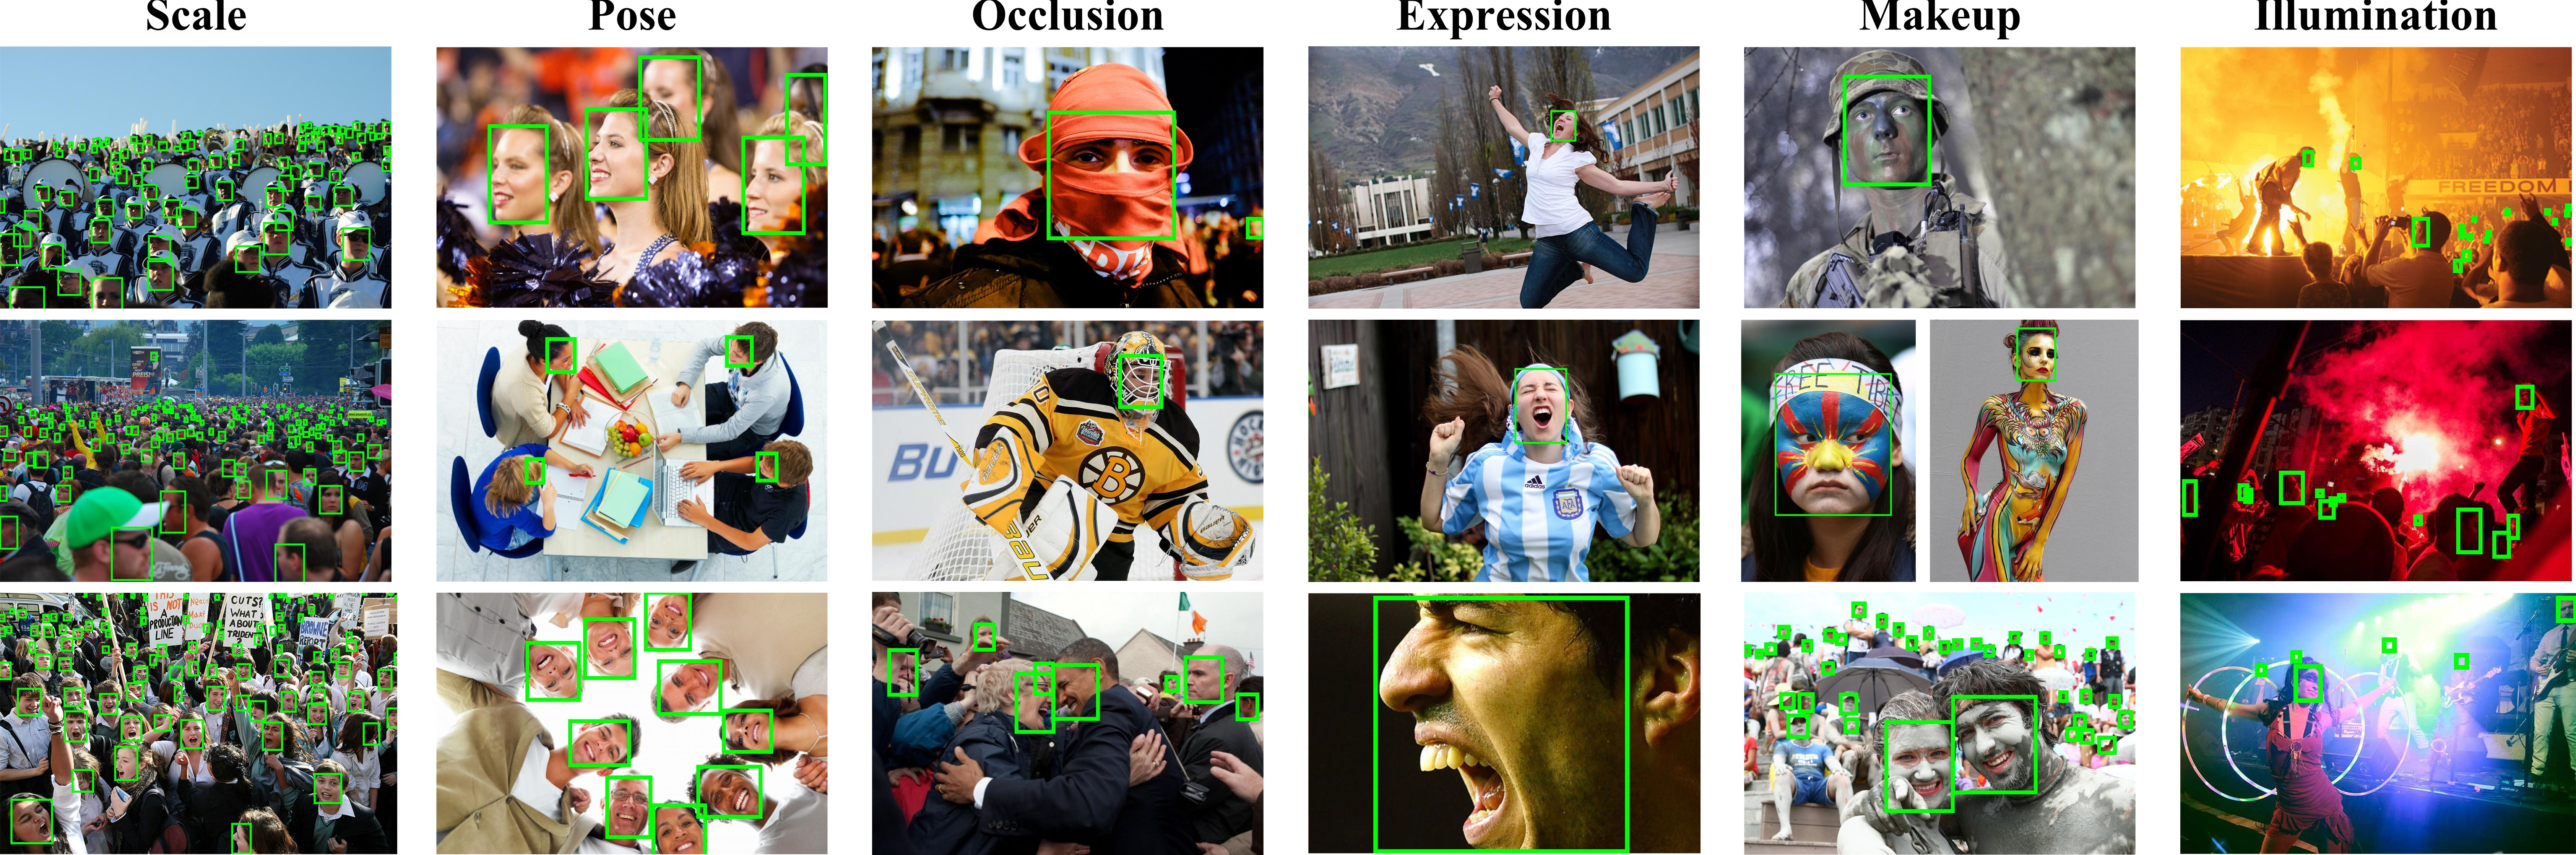
\includegraphics[width=1.0\textwidth]{bilder/wider-exampl}
    \caption{Beispiele aus dem WIDER Face Datensatz}
\end{figure} 
\subsection{Datensätze für Tensorbox bereitstellen}
\begin{enumerate}
\item Downloaden der einzelnen Datensätze Wider Face Training Images, Wider Face Validation Images und Wider Face Testing Images von der Webseiteb \url{http://mmlab.ie.cuhk.edu.hk/projects/WIDERFace/}
\item Speichern der Projekt Ordnern für die Test Bilder,$data/WIDER\_train$ für die Trainings Bilder und $data/WIDER\_val$ für die Bilder zum Validieren.
\item Der von Tensorbox benötigten Jsen Dateinen mit folgendem Konsolenbefehl:\begin{lstlisting}[language=bash] 
python wider_parser.py
\end{lstlisting}
\item Test Datensatz zusammenstellen in dem aus den zuvor erstellten Json Dateien die gewünschten Datensätze ausgewählt werden und in die $wider\_test.json$ kopiert werden.
\end{enumerate}

\section{Tensorbox}
\subsection{Installation}
\begin{enumerate}
\item Download  \url{https://github.com/DevJakobL/Face_detection}
\item Am speicherungsort folgende befehle ausführen
\begin{lstlisting}[language=bash]
	cd TENSORBOX/utils && python setup.py install && ../../
	pip install -r path/to/requirements.txt
\end{lstlisting}
\item WIDER-Face Datenbank fürs Training vorbereiten, wie in Abschnitt \ref{dataset} beschrieben.
\end{enumerate}
\subsection{Training }
\begin{lstlisting}[language=bash]
python train.py --hypes hypes/overfeat_rezoom.json --gpu 0 --logdir output
\end{lstlisting}
Mit Hilfe der hypes/overfeat\_rezoom.json Datei kann das Training für den eigenen Datensatz eingestellt werden. Mehr dazu in Abschnitt \ref{training-gesicht}.
\newpage
\subsection{Evaluation}
\begin{lstlisting}[language=bash]
python tensorbox/evaluate.py --weights WEIGHTS_FILE --test_boxes data/wider_val.jason
\end{lstlisting}
$WEIGHTS\_FILE$ beinhaltet die Gewichte des zu validierenden neuronalen Netzes \\z.B. output/overfeat\_rezoom\_2018\_07\_10\_00.50/save.ckpt-1000. Nach dem die Validierung abgeschlossen ist wird ein Ordner erstellt z.B. output/overfeat\_rezoom\_2018\_07\_10\_00.50/images\_val\_boxes\_1000. in diesem befindet sich die Ergebnis Datei "results.png" erstellt.

\chapter{Methoden}%eigene arbeit
\section{Verwendete Technologien}
\begin{itemize}
\item Python 3.7
\item Tensorbox
\end{itemize}

\section{ Struktur}
\section{Training der Gesichtserkennung }\label{training-gesicht}
\subsection{Installation von Tensorbox }
\subsection{Vorbereiten der WIDER Face Datenbank}
\subsection{Training  mittels Tensorbox}

